\documentclass[dvipdfmx]{jarticle}
\pagestyle{empty}
\newcommand{\newtemp}[1]{\texttt{newTemp(}{#1}\texttt{)}}
\newcommand{\newllabel}[1]{\texttt{newLabel(}{#1}\texttt{)}}
\newcommand{\generatetw}[2]{\texttt{generate(}{#1},=,{#2}\texttt{)}}
\newcommand{\generateth}[3]{\texttt{generate(}{#1},=,{#2},{#3}\texttt{)}}
\newcommand{\generatefo}[4]{\texttt{generate(}{#1},=,{#2},{#3},{#4}\texttt{)}}
\newcommand{\ttpl}{\texttt{+}}
\newcommand{\ttmu}{\texttt{*}}
\newcommand{\ttnum}{\texttt{NUM}}
\newcommand{\eof}{\texttt{\#}}

\newcommand{\makenewtemp}{{\tt newTemp()}}
\newcommand{\makenewlabel}{{\tt newLabel()}}
\newcommand{\gengoto}[1]{{\tt generate(`goto }{#1}{\tt ')}}
\newcommand{\genlabel}[1]{{\tt generate(`label }{#1}{\tt ')}}
\newcommand{\genifnot}[2]{{\tt generate(`if\_not}\ {#1}\ {\tt goto}\ {#2}\ {\tt ')}}
\newcommand{\genassign}[2]{{\tt generate(`}{#1}{\tt :=}{#2}{\tt ')}}
\usepackage{tikz}
\usetikzlibrary{shapes,calc}
\begin{document}
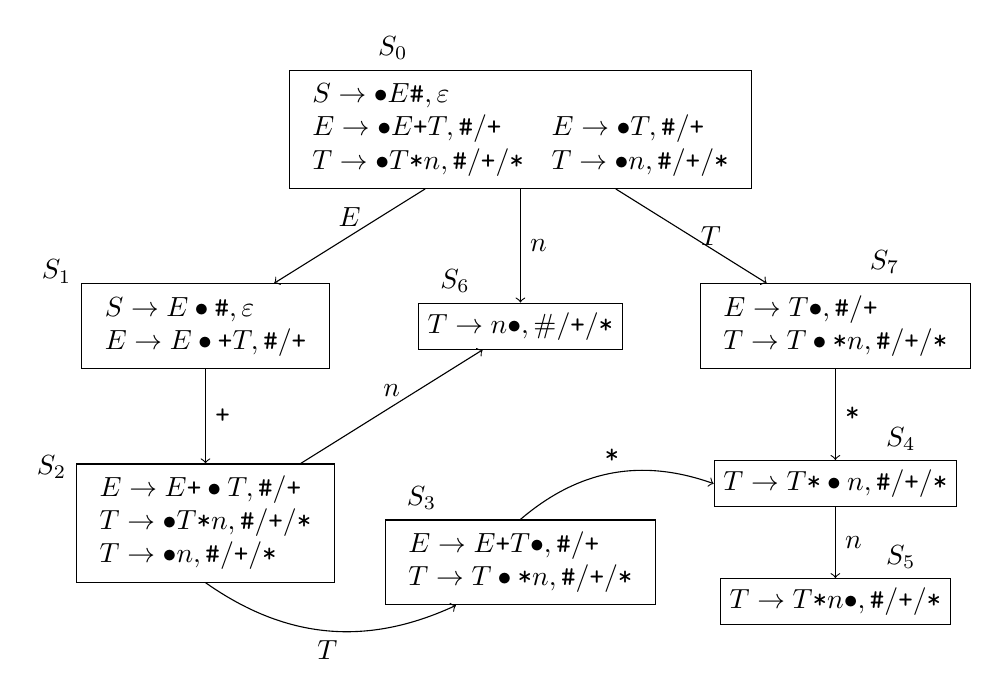
\begin{tikzpicture}
\node[draw,label={150:$S_0$}] (S0) at (0,0) {$\begin{array}{ll}
  S\rightarrow\bullet E\eof,\varepsilon\\
  E\rightarrow\bullet E\ttpl T,\eof/\ttpl &
  E\rightarrow\bullet T,\eof/\ttpl\\
  T\rightarrow\bullet T\ttmu n,\eof/\ttpl/\ttmu &
  T\rightarrow\bullet n,\eof/\ttpl/\ttmu
\end{array}$};
\node[draw,label={165:$S_1$}] (S1) at (-4,-2.5) {$\begin{array}{l}
  S\rightarrow E\bullet\eof,\varepsilon\\
  E\rightarrow E\bullet\ttpl T,\eof/\ttpl
\end{array}$};
\node[draw,label={165:$S_2$}] (S2) at (-4,-5) {$\begin{array}{l}
  E\rightarrow E\ttpl\bullet T,\eof/\ttpl\\
  T\rightarrow \bullet T\ttmu n,\eof/\ttpl/\ttmu\\
  T\rightarrow\bullet n,\eof/\ttpl/\ttmu
\end{array}$};
\node[draw,label={150:$S_6$}] (S6) at (0,-2.5) {$T\rightarrow n\bullet,\#/\ttpl/\ttmu$};
\node[draw,label={60:$S_7$}] (S7) at (4,-2.5) {$\begin{array}{l}
  E\rightarrow T\bullet,\eof/\ttpl\\
  T\rightarrow T\bullet\ttmu n,\eof/\ttpl/\ttmu
\end{array}$};
\node[draw,label={30:$S_4$}] (S4) at (4,-4.5) {$T\rightarrow T\ttmu\bullet n,\eof/\ttpl/\ttmu$};
\node[draw,label={30:$S_5$}] (S5) at (4,-6) {$T\rightarrow T\ttmu n\bullet,\eof/\ttpl/\ttmu$};
\node[draw,label={150:$S_3$}] (S3) at (0,-5.5) {$\begin{array}{l}
  E\rightarrow E\ttpl T\bullet,\eof/\ttpl\\
  T\rightarrow T\bullet\ttmu n,\eof/\ttpl/\ttmu
\end{array}$};
\path[->] (S0) edge [above] node {$E$} (S1) (S0) edge [right] node {$n$} (S6)
          (S0) edge [right] node {$T$} (S7);
\path[->] (S1) edge [right] node {$\ttpl$} (S2) (S2) edge [above] node {$n$} (S6);
\path[->] (S7) edge [right] node {$\ttmu$} (S4) (S4) edge [right] node {$n$} (S5);
\path[->] (S2.south) [bend right] edge [below] node {$T$} (S3);
\path[->] (S3.north) [bend left] edge [above] node {$\ttmu$} (S4.west);
\end{tikzpicture}
\end{document}